\documentclass[11pt]{standalone}

\usepackage{helvet}

\usepackage{ifthen}
\usepackage{tikz} 
\usetikzlibrary{shapes.misc}
\usetikzlibrary{arrows,arrows.meta}
\usetikzlibrary{calc,intersections, patterns, math}

\definecolor{bg}{RGB}{35,35,35}
\definecolor{pfeil}{RGB}{168,167,167}
\definecolor{petrol}{RGB}{0, 118, 136}
\definecolor{darkgoldenrod}{RGB}{184, 134, 11}
\colorlet{petrol-lighter}{petrol!40}
\colorlet{darkgoldenrod-lighter}{darkgoldenrod!40}

\begin{document}

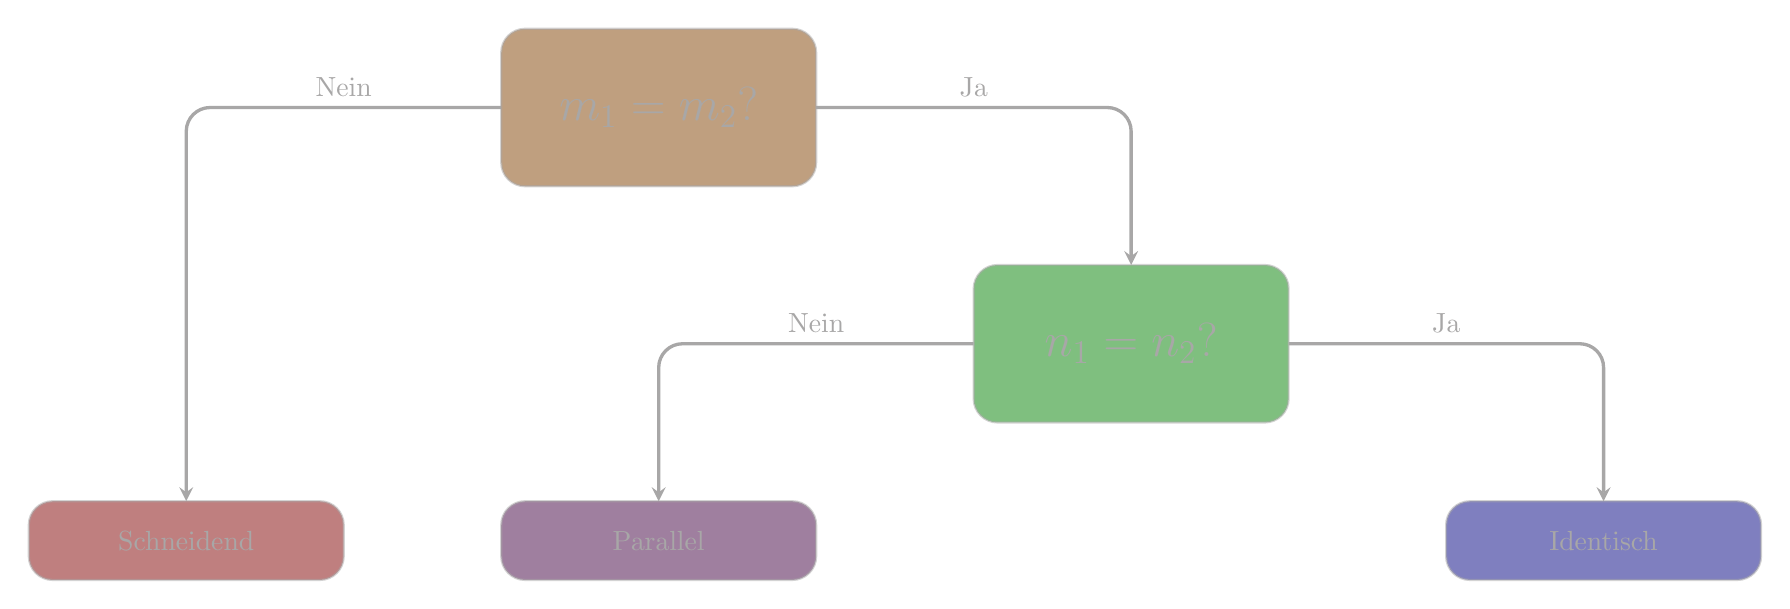
\begin{tikzpicture}[pfeil]
    % \path[fill=bg] (-10,-10) rectangle (15,3);

    % \draw[thick, fill=petrol!20, draw=petrol-lighter, rounded corners=2ex, opacity=0.5] (0,0) rectangle ++ (1.5,3.5);
    % \draw[thick, fill=darkgoldenrod!20, draw=darkgoldenrod-lighter, rounded corners=2ex, opacity=0.5] (5,0) rectangle ++ (1.5,3.5);

    \draw[thick, fill=orange!50!black, opacity=0.5, rounded corners=2ex] (-2,-1) rectangle ++(4,2);
    \node at (0,0) {\LARGE $m_1 =m_2$?};
    \draw[very thick,-stealth, rounded corners=2ex] (2,0) -- node[above] {Ja} (6,0) -- (6,-2);
    \draw[thick, fill=green!50!black, opacity=0.5, rounded corners=2ex] (4,-4) rectangle ++(4,2);
    \node at (6,-3) {\LARGE $n_1 =n_2$?};
    \draw[very thick,-stealth, rounded corners=2ex] (8,-3) -- node[above] {Ja} (12,-3) -- (12,-5);

    \draw[thick, fill=blue!50!black, opacity=0.5, rounded corners=2ex] (10,-6) rectangle ++(4,1);
    \node at (12,-5.5) {Identisch};

    \draw[very thick,-stealth, rounded corners=2ex] (4,-3) -- node[above] {Nein} (0,-3) -- (0,-5);

    \draw[thick, fill=violet!50!black, opacity=0.5, rounded corners=2ex] (-2,-6) rectangle ++(4,1);
    \node at (0,-5.5) {Parallel};

    \draw[very thick,-stealth, rounded corners=2ex] (-2,0) -- node[above] {Nein} (-6,0) -- (-6,-5);

    \draw[thick, fill=red!50!black, opacity=0.5, rounded corners=2ex] (-8,-6) rectangle ++(4,1);
    \node at (-6,-5.5) {Schneidend};

\end{tikzpicture}

\end{document}
